%instiki:category: FisicaSubatomica
\chapter{Ruptura espont\'anea de simetr\'\i a}
\label{rupt-espont-de} %noinstiki
%instiki:
%instiki:***
%instiki:
%instiki:[[NotasFS|Tabla de Contenidos]]
%instiki:
%instiki:***
%instiki:
%instiki:* [Masa para el campo escalar](#masa-para-el)
%instiki:
%instiki:* [Bos\'on de Goldstone](#boson-de-goldstone)
%instiki:
%instiki:* [Masa para el bos\'on gauge](#masa-para-el-1)
%instiki:
%instiki:* [Mecanismo de Higgs en un caso no Abeliano](#mecanismo-de-higgs)
%instiki:
%instiki:***
%instiki:


\section{Masa para el campo escalar}
\label{sec:masa-para-el}

Escribamos el Lagrangiano para una part\'\i cula escalar real de masa $m$ como
\begin{equation}
\label{eq:83}
\mathcal{L}=\tfrac{1}{2}\partial^\mu\phi\partial_\mu\phi-V(\phi)
\end{equation}
con
\begin{equation}
  V(\phi)=\tfrac{1}{2}\mu^2.
\end{equation}
Este Lagrangiano es sim\'etrico bajo la transformaci\'on discreta $\phi\to-\phi$. 

Si $\mu^2\gt 0$ el campo tiene excitaciones alrededor del m\'\i nimo del potencial que cuestan energ\'\i a y dicho t\'ermino se interpreta como la masa de la part\'\i cula. Ver figura \ref{fig:x2}. En Teor\'\i a Cu\'antica de Campos al estado de m\'\i nima energ\'\i a se le llama el vac\'\i o y las excitaciones alrededor del vaci\'o corresponden a las part\'\i culas.
%noinstiki
\begin{figure} %noinstiki
  \centering %noinstiki
  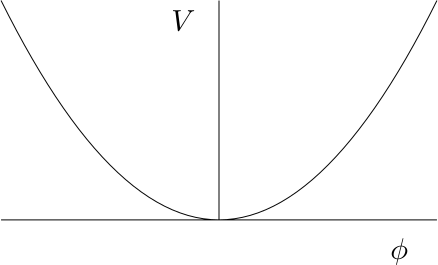
\includegraphics[scale=0.8]{vphi2}
  \caption{$V(\phi)=\frac{1}{2}\mu^2 \phi^2$ con $\mu^2\gt 0$} %noinstiki
  \label{fig:x2} %noinstiki
\end{figure} %noinstiki <div id="fig:x2">Figura: Un m\'\i nimo</div>
%noinstiki![cuerda](http://gfif.udea.edu.co/figfs/vphi2.png)
%noinstiki

Si $\mu^2\lt 0$, no existe un m\'\i nimo del potencial alrededor del cual el campo pueda oscilar. Adem\'as el alejamiento del campo del punto de simetr\'\i a del potencial no cuesta energ\'\i a. Por consiguiente en ese caso, el t\'ermino de interacci\'on
\begin{equation}
  V(\phi)=\tfrac{1}{2}\mu^2   \qquad 
  \mu^2\lt 0,
\end{equation}
no puede interpretarse como un t\'ermino de masa en el Lagrangiano dado por la ec.~\eqref{eq:83}. 

Consideremos ahora el potencial
\begin{equation}
  V(\phi)=\tfrac{1}{2}\mu^2\phi^2+\tfrac{1}{4}\lambda\phi^4
  \qquad   \mu^2\lt 0,\ \lambda\gt 0
\end{equation}
que mantiene la simetr\'\i a bajo la transformaci\'on discreta $\phi\to-\phi$. $\lambda\gt 0$ garantiza la aparici\'on de los dos m\'\i nimos que se muestran el la figura \ref{fig:x2l}. Si la energ\'\i a es suficientemente alta como se muestra en la figura~\ref{fig:x2l}, las excitaciones son sim\'etricas con respecto al m\'aximo del potencial y el t\'ermino en $\mu^2$ no puede interpretarse como masa para la part\'\i cula escalar. 

%noinstiki
\begin{figure} %noinstiki
  \centering %noinstiki
  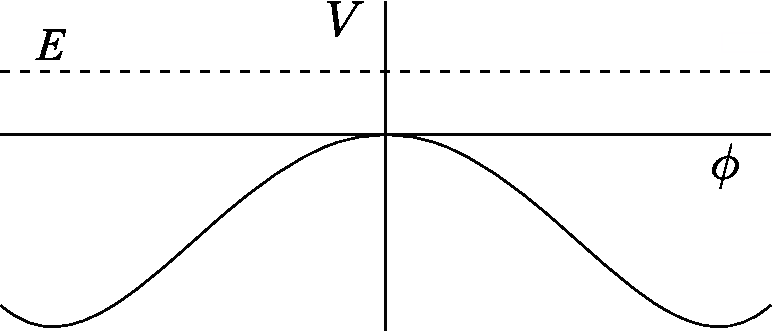
\includegraphics{vphi4}
  \caption{$V(\phi)=\frac{1}{2}\mu^2 \phi^2+\frac{1}{4}\lambda\phi^4$ con $\mu^2\lt 0$, y $\lambda\gt 0$. Simetr\'\i a ex\'acta} %noinstiki
  \label{fig:x2l} %noinstiki
\end{figure} %noinstiki <div id="fig:x2l">Figura: M\'\i nimos degenerados</div>
%noinstiki![cuerda](http://gfif.udea.edu.co/figfs/vphi4.png)
%noinstiki
Sin embargo, si la energ\'\i a es suficientemente baja como se muestra en la figura~\ref{fig:x2lm}, las excitaciones alrededor del m\'\i nimo dan lugar a la aparici\'on de un t\'ermino de masa para el campo escalar. Adem\'as, dichas excitaciones no respetan la simetr\'\i as $\phi\to-\phi$. En tal caso decimos que la simetr\'\i a ha sido espont\'aneamente rota: aunque el Lagrangiano mantiene la simetr\'\i a original, el vac\'\i o la rompe. 

%noinstiki
\begin{figure} %noinstiki
  \centering %noinstiki
  %noinstiki
  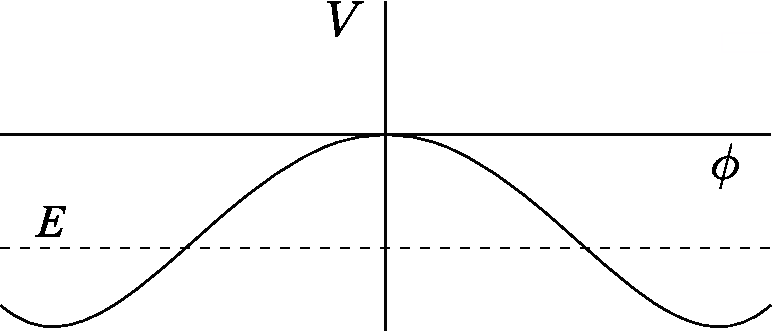
\includegraphics{vphi4m}
  \caption{$V(\phi)=\frac{1}{2}\mu^2 \phi^2+\frac{1}{4}\lambda\phi^4$ con $\mu^2\lt 0$, y $\lambda\gt 0$. Simetr\'\i a espont\'aneamente rota.} %noinstiki
  \label{fig:x2lm} %noinstiki
\end{figure}  %noinstiki <div id="fig:x2lm">Figura: Simetr\'\i a espont\'aneamente rota  </div>
%noinstiki![vphi4lm](http://gfif.udea.edu.co/figfs/vphi4lm.png)
%noinstiki

Para analizar cuantitativamente el espectro de part\'\i culas es necesario expandir el campo alrededor del m\'\i nimo y determinar las excitaciones. Establezcamos en primer lugar los m\'\i nimos del potencial. La $\partial V/\partial\phi=0$ da lugar a
\begin{align}
  \mu^2\phi+\lambda\phi^3&=0\\
  \phi(\mu^2+\lambda\phi^2)&=0,
\end{align}
con extremos $\phi_{\text{max}}=0$, y 
\begin{equation}
  \label{eq:90}
  \phi_{\text{min}}\equiv\langle\phi\rangle\equiv v=\pm\sqrt{\frac{-\mu^2}{\lambda}}.
\end{equation}
De hecho 
\begin{equation}
  \frac{\partial^2V}{\partial\phi^2}=\mu^2+3\lambda\phi^2.
\end{equation}
$\phi=0$ corresponde a un m\'aximo, mientras que la segunda derivada para $\phi=\pm\sqrt{-\mu^2/\lambda}$ es $-2\mu^2\gt 0$ y corresponden a los m\'\i nimos. Expandiendo el campo alrededor del m\'\i nimo
\begin{equation}
  \phi(x)=H(x)+v
\end{equation}
\begin{align}
  V(\phi)=&\tfrac{1}{2}\mu^2 \phi^2+\tfrac{1}{4}\lambda\phi^4\nonumber\\
  =&\tfrac{1}{2}\mu^2 (H+v)^2+\tfrac{1}{4}\lambda(H+v)^4\nonumber\\
  =&\tfrac{1}{2}\mu^2 (H+v)^2+\tfrac{1}{4}\lambda(H+v)^4\nonumber\\
  =&\tfrac{1}{2}\mu^2 \left(H^2+2vH+v^2\right)+\tfrac{1}{4}\lambda\left(H^2+2vH+v^2\right)^2\nonumber\\
  =&\tfrac{1}{2}\mu^2 \left(H^2+2vH+v^2\right)+\tfrac{1}{4}\lambda\left[H^4+2H^2\left(2vH+v^2\right)+\left(2vH+v^2\right)^2\right]\nonumber\\
  =&\tfrac{1}{2}\mu^2 \left(H^2+2vH+v^2\right)+\tfrac{1}{4}\lambda\left[H^4+4vH^3+2H^2v^2+4v^2H^2+4v^3H+v^4\right]\nonumber\\
  =&\tfrac{1}{2}\mu^2 \left(H^2+2vH+v^2\right)+\tfrac{1}{4}\lambda\left[H^4+4vH^3+6H^2v^2+4v^3H+v^4\right]\nonumber\\
  =&\tfrac{1}{2}\mu^2H^2-\tfrac{3}{2}H^2\mu^2+\mu^2vH-\mu^2vH+\tfrac{1}{2}\mu^2v^2-\tfrac{1}{4}\mu^2v^2+\tfrac{1}{4}\lambda\left[H^4+4vH^3\right]\nonumber\\
\label{eq:84}
V(H)=&\tfrac{1}{2}\left(-2\mu^2\right)H^2+\lambda vH^3+\tfrac{1}{4}\lambda H^4+\tfrac{1}{4}\mu^2v^2,
\end{align}
y
\begin{equation}
  \label{eq:88}
  \mathcal{L}_H=\tfrac{1}{2}\partial^\mu H\partial_\mu H-\tfrac{1}{2}\left(-2\mu^2\right)H^2-\lambda vH^3-\tfrac{1}{4}\lambda H^4+\text{constant}.
\end{equation}
Entonces $H$ adquiere una masa $-2\mu^2$ y no es invariante bajo $H\to-H$. 

Otro m\'etodo es usar las ecuaciones de m\'\i nimo $-\mu^2=\lambda v^2$, para eliminar un par\'ametro del potencial:
\begin{align}
  V(\phi)&=-\tfrac{1}{2}\lambda v^2\phi^2+\tfrac{1}{4}\lambda\phi^4\nonumber\\
  =&-\tfrac{1}{2}\lambda v^2 \left(H^2+2vH+v^2\right)+\tfrac{1}{4}\lambda\left[H^4+4vH^3+6H^2v^2+4v^3H+v^4\right]\nonumber\\
  =&\lambda v^2H^2+\lambda vH^3+\tfrac{1}{4}\lambda H^4+\text{constant}.
\end{align}

\section{Bos\'on de Goldstone}
\label{sec:boson-de-goldstone}

Consideremos ahora un campo escalar complejo sin t\'ermino de masa, pero con potencial:
\begin{equation}
  \label{eq:85}
  \mathcal{L}=\partial^\mu\phi^*\partial_\mu\phi-V(\phi)
\end{equation}
\begin{equation}
  V(\phi)=\mu^2\phi^*\phi+\lambda(\phi^*\phi)^2 
  \qquad 
  \mu^2\lt 0,\ \lambda\gt 0 
\end{equation}
La simetr\'\i a del Lagrangiano corresponde a $U(1)$ global. Este potencial corresponde al ``sombrero mexicano''. Para una energ\'\i a suficientemente baja de manera que el campo deba oscilar alrededor del m\'\i nimo aparecen dos tipos de excitaciones. Una sobre las paredes  que cuestan energ\'\i a y corresponden a un campo escalar cargado como en el caso anterior, y otra a lo largo de la circunferencia de m\'\i nimo, que corresponde a una part\'\i cula escalar sin masa.
 

Anal\'\i ticamente tenemos dos formar de abordar el an\'alisis

\subsection{Coordenadas cartesianas}
Expandimos el campo alrededor del m\'\i nimo:

\begin{equation}
  \label{eq:193}
  \phi=\phi^0=\frac{\phi_1+i\phi_2}{\sqrt{2}}=\frac{1}{\sqrt{2}}(H(x)+v+iG)
\end{equation}
Entonces
\begin{align}
  \label{eq:194}
  V(\phi_1,\phi_2)=\tfrac{1}{2}\mu^2\left(\phi_1^2+\phi_2^2\right)
+\tfrac{1}{4}\lambda\left(\phi_1^2+\phi_2^2\right)^2
\end{align}
%\left(\right)
La condici\`on de m\'\i nimo es 
\begin{align}
  \frac{\partial V}{\partial\phi_1}=&0\nonumber\\
  =&\tfrac{1}{2}\mu^2\left(2\phi_1\right)
+\tfrac{1}{4}\lambda2\left(\phi_1^2+\phi_2^2\right)2\phi_1\nonumber\\
  =&\phi_1\left[\mu^2+\lambda\left(\phi_1^2+\phi_2^2\right)\right]
\end{align}
\begin{align}
  \frac{\partial V}{\partial\phi_2}=&0\nonumber\\
  =&\phi_2\left[\mu^2+\lambda\left(\phi_1^2+\phi_2^2\right)\right]
\end{align}
Los infinitos m\'\i nimos degenerados corresponden a la circunferencia
\begin{equation}
\phi_1^2+\phi_2^2=v^2=\frac{-\mu^2}{\lambda}
\end{equation}
El campo debe ser neutro pues, reemplazando \eqref{eq:193} en la ec.~\eqref{eq:194}
\begin{align}
  \mathcal{L}=&\tfrac{1}{2}\partial^\mu H\partial_\mu H+\tfrac{1}{2}\partial^\mu G\partial_\mu G-\tfrac{1}{2}\mu^2\left[(H+v)^2+G^2\right]-\tfrac{1}{4}\lambda\left[(H+v)^4+2(H+v)^2G^2+G^4\right]\nonumber\\
  \mathcal{L}=&\tfrac{1}{2}\partial^\mu H\partial_\mu H-\tfrac{1}{2}\mu^2(H+v)^2-\tfrac{1}{4}\lambda(H+v)^4+\tfrac{1}{2}\partial^\mu G\partial_\mu G-\tfrac{1}{2}\mu^2G^2-\tfrac{1}{4}\lambda\left[2(H+v)^2G^2+G^4\right].
\end{align}
Usando la ec.~(\ref{eq:84}), tenemos
\begin{align}
  \mathcal{L}=&\tfrac{1}{2}\partial^\mu H\partial_\mu H-\tfrac{1}{2}\left(-2\mu^2\right)H^2-\lambda vH^3-\tfrac{1}{4}\lambda H^4\nonumber\\
  &+\tfrac{1}{2}\partial^\mu G\partial_\mu G-\tfrac{1}{2}\mu^2G^2-\tfrac{1}{4}\lambda G^4\nonumber\\
  &-\tfrac{1}{2}\lambda\left[H^2G^2+2vHG^2+v^2G^2\right]+\text{constant}\nonumber\\
\end{align}
\begin{align}
    \mathcal{L}=&\tfrac{1}{2}\partial^\mu H\partial_\mu H-\tfrac{1}{2}\left(-2\mu^2\right)H^2-\lambda vH^3-\tfrac{1}{4}\lambda H^4\nonumber\\
  &+\tfrac{1}{2}\partial^\mu G\partial_\mu G-\tfrac{1}{4}\lambda G^4\nonumber\\
  &-\lambda vHG^2-\tfrac{1}{2}\lambda H^2G^2+\text{constant}\nonumber\\
\end{align}
Como antes, el campo $H$ tiene masa $2|\mu^2|$. El t\'ermino en $G^2$ ha desaparecido implicando que el campo $G$ tiene masa cero.
En este caso decimos que la invarianza $U(1)$ de la acci\'on ha sido espont\'aneamente rota
\begin{equation}
  U=e^{iY\theta},
\end{equation}
donde $Y$ es el generador de la transformaci\'on y $\theta$ el par\'ametro. Despu\'es de la ruptura espont\'anea de la simetr\'\i a diremos que el generador $Y$ ha sido roto. El campo que adquiere masa recibe el nombre de \emph{bos\'on de Higgs} \cite{Higgs:1964pj}, mientras que el campo sin masa es llamado \emph{bos\'on de Goldstone}. 

El \emph{Teorema de Goldstone} establece que por cada generador roto de una simetr\'\i a continua debe aparecer un bos\'on de Goldstone.

\subsection{Coordenadas polares}

Si hacemos
\begin{equation}
  \phi=e^{i\eta(x)}\frac{\rho(x)}{\sqrt{2}}
\end{equation}
\begin{align}
  \mathcal{L}&=\tfrac{1}{2}\left(\partial^\mu\rho-i\rho\partial^\mu\eta\right)\left(\partial_\mu\rho+i\rho\partial_\mu\eta\right)-\tfrac{1}{2}\mu^2\rho^2-\tfrac{1}{2}\lambda\rho^4\nonumber\\
    \mathcal{L}&=\tfrac{1}{2}\partial^\mu\rho\partial_\mu\rho+\tfrac{1}{2}\rho^2\partial^\mu\eta\partial_\mu\eta-\tfrac{1}{2}\mu^2\rho^2-\tfrac{1}{2}\lambda\rho^4
\end{align}


Haciendo $\rho\to \rho+v$, tenemos
\begin{align}
  \mathcal{L}=&\tfrac{1}{2}\partial^\mu\rho\partial_\mu\rho-\tfrac{1}{2}\mu^2(\rho+v)^2-\tfrac{1}{2}\lambda(\rho+v)^4\nonumber\\
  +&\tfrac{1}{2}v^2\partial^\mu\eta\partial_\mu\eta+\tfrac{1}{2}\rho^2\partial^\mu\eta\partial_\mu\eta+2v\rho\partial^\mu\eta\partial_\mu\eta\nonumber\\
  \mathcal{L}=&\tfrac{1}{2}\partial^\mu\rho\partial_\mu\rho-\tfrac{1}{2}\left(-2\mu^2\right)\rho^2-\lambda v\rho^3-\tfrac{1}{4}\lambda \rho^4\nonumber\\
  +&\tfrac{1}{2}v^2\partial^\mu\eta\partial_\mu\eta+\tfrac{1}{2}\rho^2\partial^\mu\eta\partial_\mu\eta+2v\rho\partial^\mu\eta\partial_\mu\eta
\end{align}
De nuevo no hay t\'ermino de masa para $\eta$.

\section{Masa para el bos\'on gauge}
\label{sec:masa-para-el-1}
En el caso de la Acci\'on invariante gauge local bajo el Grupo $U(1)$, tenemos el Lagrangiano \eqref{eq:56}:
\begin{equation}
  \label{eq:89}
  \mathcal{L}=\left(\mathcal{D}^\mu\phi\right)^*\mathcal{D}_\mu\phi-\mu^2\phi^*\phi-\lambda\left(\phi^*\phi\right)^2-\tfrac{1}{4}F^{\mu\nu}F_{\mu\nu}
  \qquad 
  \mu^2\lt 0\text{ and } \lambda\gt 0
\end{equation}
Para obtener directamente el espectro despu\'es de la ruptura espont\'anea de simetr\'\i a es conveniente usar la transformaci\'on gauge de la ec.~\eqref{eq:86}. Haciendo $\theta(x)=-\eta(x)$:
\begin{equation}
\label{eq:87}
   \phi\to\phi'=e^{i\theta(x)}e^{i\eta(x)}\left(\frac{H(x)+v}{\sqrt{2}}\right)=\frac{H(x)+v}{\sqrt{2}}
\end{equation}
\begin{align}
  \mathcal{L}\to\mathcal{L}' &=\left[\left(\mathcal{D}^\mu\right)'\phi'\right]^*\left(\mathcal{D}_\mu\right)'\phi'-\mu^2\left(\phi^*\right)'\phi'-\lambda\left[\left(\phi^*\right)'\phi'\right]^2-\tfrac{1}{4}\left(F^{\mu\nu}F_{\mu\nu}\right)'\nonumber\\
 &=\tfrac{1}{2}\left[\partial^\mu H+ig{A'}^\mu(H+v)\right]\left[\partial_\mu H-ig{A'}_\mu(H+v)\right]-\tfrac{1}{2}\mu^2(H+v)^2-\tfrac{1}{4}\lambda(H+v)^4-\tfrac{1}{4}F^{\mu\nu}F_{\mu\nu}
\end{align}
En adelante omitiremos las primas, aunque debe estar claro que se esta trabajando en el gauge espec\'\i fico de la ec.~\eqref{eq:87}. Entonces
\begin{align}
  \mathcal{L}&=\tfrac{1}{2}\partial^\mu H\partial_\mu H-\tfrac{1}{2}\mu^2(H+v)^2-
  \tfrac{1}{4}\lambda(H+v)^4+\tfrac{1}{2}g^2A^\mu A_\mu(H+v)^2
  -\tfrac{1}{4}F^{\mu\nu}F_{\mu\nu}.
\end{align}
Usando la ec.~\eqref{eq:84}
\begin{equation}
  \label{eq:94}
  \mathcal{L}=\mathcal{L}_H+\mathcal{L}_{A^\mu}+\tfrac{1}{2}g^2A^\mu A_\mu H^2+g^2vA^\mu A_\mu H,
\end{equation}
donde $\mathcal{L}_H$ esta dado por la ec.~\eqref{eq:88} y
\begin{equation}
  \mathcal{L}_{A^\mu}=-\tfrac{1}{4}F^{\mu\nu}F_{\mu\nu}+\tfrac{1}{2}g^2v^2A^\mu A_\mu.
\end{equation}
Teniendo en cuenta la ec.~\eqref{eq:23} para el Lagrangiano de Proca, vemos que como consecuencia de la ruptura espont\'anea de simetr\'\i a el campo gauge ha adquirido una masa
\begin{equation}
  m_{A^\mu}=gv.
\end{equation}

El mecanismo completo mediante el cual, a partir de un Lagrangiano invariante gauge local, los bosones gauge adquieren masa se llama \emph{mecanismo de Higgs} \cite{Higgs:1964pj}. La part\'\i cula escalar que adquiere masa se llama Higgs, mientras que el bos\'on de Goldstone es absorbido por campo gauge como modo longitudinal. 

El n\'umero de grados de libertad independientes en el Lagrangiano original en la ec.~\eqref{eq:89} es cuatro. Correspondientes a los dos grados de libertad del bos\'on gauge no masivo y los dos del campo escalar complejo. En el Lagrangiano final en la ec.~\eqref{eq:94} no aparece el bos\'on de Goldstone. Sin embargo esto no es un problema porque dicho Lagrangiano tambi\'en tiene cuatro grados de libertad correspondientes a  los tres grados de libertad del bos\'on gauge masivo y al grado de libertad del bos\'on de Higgs. 

Sin usar la transformaci\'on gauge en ec.~\eqref{eq:89}, tenemos que para
\begin{equation}
  \phi=\frac{1}{\sqrt{2}}\left(H(x)+v+iG(x)\right)
\end{equation}
\begin{align}
  \mathcal{L}=&\tfrac{1}{2}\left[\partial^\mu H-i\partial^\mu G+igA^\mu(H+v)+gA^\mu G\right]\left[\partial_\mu H+i\partial_\mu G-igA_\mu(H+v)+gA_\mu G\right]\nonumber\\
&-\tfrac{1}{2}\mu^2(H+v)^2-\tfrac{1}{2}\mu^2G^2-\tfrac{1}{4}\lambda(H+v)^4-\tfrac{1}{4}\lambda G^4-\tfrac{1}{2}\lambda G^2(H+v)^2-\tfrac{1}{4}F^{\mu\nu}F_{\mu\nu}\nonumber\\
=&\tfrac{1}{2}\left\{\partial^\mu H+gA^\mu G+i\left[-\partial^\mu G+gA^\mu(H+v)\right]\right\}\left\{\partial_\mu H+gA_\mu G-i\left[-\partial_\mu G+igA_\mu(H+v)\right]\right\}\nonumber\\
&-\tfrac{1}{2}\mu^2(H+v)^2-\tfrac{1}{2}\mu^2G^2-\tfrac{1}{4}\lambda(H+v)^4-\tfrac{1}{4}\lambda G^4-\tfrac{1}{2}\lambda G^2(H^2+2vH+v^2)-\tfrac{1}{4}F^{\mu\nu}F_{\mu\nu}\nonumber\\
=&\tfrac{1}{2}\left(\partial^\mu H+gA^\mu G\right)^2+\tfrac{1}{2}\left[-\partial^\mu G+gA^\mu(H+v)\right]^2\nonumber\\
&-\tfrac{1}{2}\mu^2(H+v)^2-\tfrac{1}{4}\lambda(H+v)^4-\tfrac{1}{4}\lambda G^4-\tfrac{1}{2}\lambda G^2(H^2+2vH)-\tfrac{1}{4}F^{\mu\nu}F_{\mu\nu}\nonumber\\
=&\tfrac{1}{2}\partial^\mu H\partial_\mu H-\tfrac{1}{2}\mu^2(H+v)^2-\tfrac{1}{4}\lambda(H+v)^4-\tfrac{1}{4}F^{\mu\nu}F_{\mu\nu}\nonumber\\
&-\tfrac{1}{4}\lambda G^4-g\partial^\mu GA_\mu H+\tfrac{1}{2}g^2A^\mu A_\mu H^2+g^2vA^\mu A_\mu H+g\partial^\mu HA_\mu G\nonumber\\
&+\tfrac{1}{2}g^2A^\mu A_\mu G^2-\tfrac{1}{2}\lambda G^2(H^2+2vH)\nonumber\\
&+\tfrac{1}{2}\partial^\mu G\partial_\mu G+\tfrac{1}{2}g^2v^2A^\mu A_\mu-gv\partial^\mu GA_\mu\nonumber\\
=&\mathcal{L}_H-\tfrac{1}{4}F^{\mu\nu}F_{\mu\nu}+\mathcal{L}_{\text{int}}+\mathcal{L}_2,
\end{align}
donde
\begin{align}
\mathcal{L}_{\text{int}}=&-\tfrac{1}{4}\lambda G^4-g\partial^\mu GA_\mu H+\tfrac{1}{2}g^2A^\mu A_\mu H^2+g^2vA^\mu A_\mu H+g\partial^\mu HA_\mu G\nonumber\\
&+\tfrac{1}{2}g^2A^\mu A_\mu G^2-\tfrac{1}{2}\lambda G^2(H^2+2vH)\nonumber\\
\mathcal{L}_2=&\tfrac{1}{2}\partial^\mu G\partial_\mu G+\tfrac{1}{2}g^2v^2A^\mu A_\mu-gv\partial^\mu GA_\mu
\end{align}
Podemos interpretar  $\mathcal{L}_2$ como los t\'erminos de mezcla entre $A^\mu$ y, para compensar el \'\i ndice de Lorentz, $\partial^\mu G$. Podemos escribirlo en  forma matricial como
\begin{align}
  \mathcal{L}_2=&\tfrac{1}{2}
  \begin{pmatrix}
    \partial^\mu G & A^\mu    
  \end{pmatrix}
  \begin{pmatrix}
    1   & -gv\\
    -gv & g^2v^2
  \end{pmatrix}
  \begin{pmatrix}
    \partial_\mu G\\
    A_\mu
  \end{pmatrix}
\end{align}
Sea
\begin{equation}
  V=\begin{pmatrix}
    \cos\beta & \sin\beta\\
    -\sin\beta& \cos\beta
  \end{pmatrix}
\end{equation}
con $\tan\beta=1/(gv)$. Si
\begin{equation}
   \begin{pmatrix}
    \partial_\mu G\\
    A_\mu
  \end{pmatrix}=V^T \begin{pmatrix}
    \partial_\mu G'\\
    A'_\mu
  \end{pmatrix},
\end{equation}
\begin{align}
  \mathcal{L}_2=&\tfrac{1}{2}
  \begin{pmatrix}
    \partial^\mu G' & {A'}^\mu    
  \end{pmatrix}\left[V
  \begin{pmatrix}
    1   & -gv\\
    -gv & g^2v^2
  \end{pmatrix}V^T\right]
  \begin{pmatrix}
    \partial_\mu G'\\
    A'_\mu
  \end{pmatrix}\nonumber\\
  =&\tfrac{1}{2}
  \begin{pmatrix}
    \partial^\mu G' & {A'}^\mu    
  \end{pmatrix}
  \begin{pmatrix}
    0   & 0\\
    0 & 1+g^2v^2
  \end{pmatrix}
  \begin{pmatrix}
    \partial_\mu G'\\
    A'_\mu
  \end{pmatrix}\nonumber\\
  =&\tfrac{1}{2}\left(1+g^2v^2\right){A'}^\mu A'_\mu.
\end{align}
De nuevo, el bos\'on de Goldstone, en este caso $\partial^\mu G'$, es absorbido como modo longitudinal del $A'_\mu$.

\section{Mecanismo de Higgs en un caso no Abeliano}
\label{sec:mecanismo-de-higgs}

Consideremos ahora una Acci\'on invariante gauge local bajo $S(2)\times U(1)_Y$. Esta corresponde al sector bos\'onico del Modelo Est\'andar de las part\'\i culas elementales. Generalizando el Lagrangiano en la ec.~\eqref{eq:91}
\begin{equation}
\label{eq:97}
  \mathcal{L}=\left(\mathcal{D}^\mu\Phi\right)^\dagger\mathcal{D}_\mu\Phi-\mu^2\Phi^\dagger \Phi-\lambda\left(\Phi^\dagger \Phi\right)^2-\tfrac{1}{2}\operatorname{Tr}\left(W^{\mu\nu}W_{\mu\nu}\right)-\tfrac{1}{4}B^{\mu\nu}B_{\mu\nu},
\end{equation}
con $\mu^2\lt 0$ y $\lambda\gt 0$. Adem\'as
\begin{equation}
\label{eq:93}
  \Phi\overset{SU(2)\times U(1)_Y}{\longrightarrow}\Phi'=e^{i(\theta_jT^j+\alpha Y\cdot I)}\Phi,
\end{equation}
y
\begin{align}
\mathcal{D}_\mu&=I\cdot\partial_\mu-i g W_\mu-i g' Y B_\mu=I\cdot\partial_\mu-i g T_i W_\mu^i-i g' Y B_\mu.
\end{align}
De la ec.\eqref{eq:71}
\begin{align}
      W_\mu=T_i W^{i}_\mu=\begin{pmatrix}
    \frac{1}{2}W_3&\frac{1}{\sqrt{2}}W^+_\mu\\
    \frac{1}{\sqrt{2}}W^-_\mu&-\frac{1}{2}W^3_\mu
  \end{pmatrix}.
\end{align}
De modo que
\begin{align}
 \mathcal{D}_\mu &=  \begin{pmatrix}
    \partial_\mu-i\left(\frac{1}{2}g W^3_\mu+g' Y B_\mu\right)&-\frac{i}{\sqrt{2}}g W^+_\mu\\
    -\frac{i}{\sqrt{2}}g W^-_\mu&\partial_\mu-i\left(-\frac{1}{2}g W^3_\mu+g'Y B_\mu\right)
  \end{pmatrix}.
\end{align}
Sin perdida de generalidad los cuatro grados de libertad de $\Phi$, pueden escribirse en la forma
\begin{align}
\label{eq:92}
  \Phi=&e^{i\eta_jT^j}
  \begin{pmatrix}
    0\\
    \frac{1}{\sqrt{2}}(H(x)+v)
  \end{pmatrix}\\
  \approx&
  \frac{1}{2}\begin{pmatrix}
    1+i\eta_3&\sqrt{2}i\eta^+\\
    \sqrt{2}i\eta^-&1-i\eta_3
  \end{pmatrix}  \begin{pmatrix}
    0\\
    \frac{1}{\sqrt{2}}(H(x)+v)
  \end{pmatrix}\nonumber\\
  =&\frac{1}{2}\begin{pmatrix}
    i\eta^+H+vi\eta^+\\
    \frac{1}{\sqrt{2}}(H+v-i\eta_3H-i)
  \end{pmatrix}\nonumber\\
  =&\begin{pmatrix}
    G^+\\
    \frac{1}{\sqrt{2}}(h+v-iG^0)
  \end{pmatrix}.\nonumber
\end{align}
Para $SU(2)\times U(1)_Y$ tenemos cuatro generadores y cuatro bosones gauge. De acuerdo a la parametrizaci\'on en ec.~\eqref{eq:92} esperamos que aparezcan tres bosones de Goldstone, de manera que quedar\'a un generador no roto correspondiente a una simetr\'\i a remanente del vac\'\i o $U(1)_Q$
\begin{equation}
  SU(2)\times U(1)_Y\overset{\langle\Phi\rangle}{\longrightarrow}U(1)_Q.
\end{equation}
Se espera entonces que el espectro consista de un bos\'on de Higgs, tres bosones gauge masivos, y un bos\'on gauge sin masa.

Para $\alpha=0$, podemos hacer una transformaci\'on gauge usando la ec.~\eqref{eq:93} sobre el campo $\Phi$, tal que
\begin{equation}
  \label{eq:123}
    \Phi\to\Phi'=
  \begin{pmatrix}
    0\\
    \frac{1}{\sqrt{2}}(H(x)+v)
  \end{pmatrix},
\end{equation}
que define el \emph{gauge unitario}. En adelante sin embargo omitiremos las primas sobre los campos transformados $\Phi'$ y $W'_{\mu\nu}$.
\begin{equation}
  \mathcal{L}=\frac{1}{2}\left[\mathcal{D}^\mu \begin{pmatrix}
    0\\
    H(x)+v
  \end{pmatrix}\right]^\dagger\mathcal{D}_\mu\begin{pmatrix}
    0\\
    H(x)+v
  \end{pmatrix}-V(H)-\tfrac{1}{2}\operatorname{Tr}\left(W^{\mu\nu}W_{\mu\nu}\right)-\tfrac{1}{4}B^{\mu\nu}B_{\mu\nu},
\end{equation}
donde $V(H)$ dado en la ec.~\eqref{eq:84}, incluye el t\'ermino de masa para el bos\'on de Higgs
\begin{equation}
  m_H^2=2\left|\mu^2\right|=2\lambda v^2
\end{equation}
\begin{align}
  \mathcal{L}=&\frac{1}{2}\left[\begin{pmatrix}
    -\frac{i}{\sqrt{2}}g{W^\mu}^+(H+v)\\
    \partial^\mu H-i\left(-\frac{1}{2}gW_3^\mu+g'Y_\Phi B^\mu\right)(H+v)
  \end{pmatrix}\right]^\dagger\begin{pmatrix}
    -\frac{i}{\sqrt{2}}gW_\mu^+(H+v)\\
    \partial_\mu H-i\left(-\frac{1}{2}gW^3_\mu+g'Y_\Phi B_\mu\right)(H+v)
  \end{pmatrix}\nonumber\\
  &-V(H)-\tfrac{1}{2}\operatorname{Tr}\left(W^{\mu\nu}W_{\mu\nu}\right)-\tfrac{1}{4}B^{\mu\nu}B_{\mu\nu}\nonumber\\
=&\frac{1}{2}\begin{pmatrix}
    \frac{i}{\sqrt{2}}g{W^\mu}^-(H+v)&
    \partial^\mu H+i\left(-\frac{1}{2}gW_3^\mu+g'Y_\Phi B^\mu\right)(H+v)
  \end{pmatrix}\cdot\nonumber\\
  &\begin{pmatrix}
    -\frac{i}{\sqrt{2}}gW_\mu^+(H+v)\\
    \partial_\mu H-i\left(-\frac{1}{2}gW^3_\mu+g'Y_\Phi B_\mu\right)(H+v)
  \end{pmatrix}\nonumber\\
  &-V(H)-\tfrac{1}{2}\operatorname{Tr}\left(W^{\mu\nu}W_{\mu\nu}\right)-\tfrac{1}{4}B^{\mu\nu}B_{\mu\nu}\nonumber\\
  =&\frac{1}{4}g^2{W^\mu}^-W_\mu^+(H+v)^2\nonumber\\
  &+\frac{1}{2}\left[\partial^\mu H+i\left(-\tfrac{1}{2}gW_3^\mu+g'Y_\Phi B^\mu\right)(H+v)\right]\left[\partial_\mu H-i\left(-\tfrac{1}{2}gW^3_\mu+g'Y_\Phi B_\mu\right)(H+v)\right]\nonumber\\
  &-V(H)-\tfrac{1}{2}\operatorname{Tr}\left(W^{\mu\nu}W_{\mu\nu}\right)-\tfrac{1}{4}B^{\mu\nu}B_{\mu\nu}\nonumber\\
 =&\frac{1}{2}\partial^\mu H\partial_\mu H-V(H)-\tfrac{1}{2}\operatorname{Tr}\left(W^{\mu\nu}W_{\mu\nu}\right)-\tfrac{1}{4}B^{\mu\nu}B_{\mu\nu}\nonumber\\
  &+\frac{1}{4}g^2{W^\mu}^-W_\mu^+(H+v)^2+\frac{1}{2}\left(-\tfrac{1}{2}gW_3^\mu+g'Y_\Phi B^\mu\right)^2(H+v)^2
\end{align}
Entonces

\begin{align}
  \mathcal{L}=&\frac{1}{2}\partial^\mu H\partial_\mu H-V(H)-\tfrac{1}{4}W^{\mu\nu}_iW_{\mu\nu}^i-\tfrac{1}{4}B^{\mu\nu}B_{\mu\nu}\nonumber\\
  \label{eq:96}
  &+\left(\frac{gv}{4}\right)^2{W^\mu}^-W_\mu^++\frac{1}{4}g^2{W^\mu}^-W_\mu^+H^2+\frac{1}{2}vg^2{W^\mu}^-W_\mu^+H+\mathcal{L}_{WB}
\end{align}

\begin{align}
  \mathcal{L}_{WB}=\frac{1}{2}\left(\tfrac{1}{4}g^2W_3^\mu W^3_\mu-\tfrac{1}{2}gg'Y_\Phi W_3^\mu B_\mu-\tfrac{1}{2}gg'Y_\Phi W_3^\mu B_\mu+{g'}^2Y_\Phi ^2B^\mu B_\mu\right)^2\left(H^2+2vH+v^2\right)
\end{align}
Haciendo $Y_\Phi =1/2$ como en la ec.~\eqref{eq:196},
\begin{align}
  \mathcal{L}_{WB}=\frac{1}{8}
  \begin{pmatrix}
    W^\mu_3 & B^\mu
  \end{pmatrix}
  \begin{pmatrix}
    g^2&-gg'\\
    -gg'&{g'}^2
  \end{pmatrix}
  \begin{pmatrix}
    W^3_\mu\\
    B_\mu
  \end{pmatrix}
\left(H^2+2vH+v^2\right)
\end{align}
Sea
\begin{equation}
  V=\begin{pmatrix}
    \cos\theta_W & \sin\theta_W\\
    -\sin\theta_W& \cos\theta_W
  \end{pmatrix}=
  \frac{1}{\sqrt{g^2+{g'}^2}}\begin{pmatrix}
    g   & g'\\
    -g' & g
  \end{pmatrix},
\end{equation}
con $\tan\theta_W=g'/g$, tal que $g\sin\theta_W=g'\cos\theta_W$, como en la ec.~\eqref{eq:82}. Si (ver ec.~\eqref{eq:81}),
\begin{equation}
  \begin{pmatrix}
    W^3_\mu\\
    B_\mu
  \end{pmatrix}=V
  \begin{pmatrix}
    Z_\mu\\
    A_\mu
  \end{pmatrix}
\end{equation}
entonces
\begin{align}
  \mathcal{L}_{WB}=\frac{1}{8}
  \begin{pmatrix}
    Z^\mu & A^\mu
  \end{pmatrix}\left[V^T
  \begin{pmatrix}
    g^2&-gg'\\
    -gg'&{g'}^2
  \end{pmatrix}V\right]
  \begin{pmatrix}
    Z_\mu\\
    A_\mu
  \end{pmatrix}
\left(H^2+2vH+v^2\right)
\end{align}
\begin{align}
  V^T
  \begin{pmatrix}
    g^2&-gg'\\
    -gg'&{g'}^2
  \end{pmatrix}V=&\frac{1}{g^2+{g'}^2}
  \begin{pmatrix}
    g^3+g{g'}^2 & -g^2g'-{g'}^3\\
+g^2g'-g^2g'    &-g{g'}^2+g{g'}^2
  \end{pmatrix}
\begin{pmatrix}
    g   & g'\\
    -g' & g
  \end{pmatrix}\nonumber\\
=&\frac{1}{g^2+{g'}^2}
  \begin{pmatrix}
    g^3+g{g'}^2 & -g^2g'-{g'}^3\\
    0   &0
  \end{pmatrix}
\begin{pmatrix}
    g   & g'\\
    -g' & g
  \end{pmatrix}\nonumber\\
=&\frac{1}{g^2+{g'}^2}
  \begin{pmatrix}
    g^4+g^2{g'}^2+g^2{g'}^2+{g'}^4 & g^3g'+g{g'}^3-g^3g'-g{g'}^3\\
    0    &0
  \end{pmatrix}\nonumber\\
=&\begin{pmatrix}
    g^2+{g'}^2 & 0\\
    0    &0
  \end{pmatrix}
\end{align}


\begin{align}
  \mathcal{L}_{WB}&=\frac{1}{2}\left(\frac{g^2+{g'}^2}{4}\right)Z^\mu Z_\mu
  \left(H^2+2vH+v^2\right)\nonumber\\
  &=\frac{1}{2}\left(\frac{g}{2}\right)^2\left(1+\tan^2\theta_W\right)Z^\mu Z_\mu\left(H^2+2vH+v^2\right)\nonumber\\
  &=\frac{1}{2}\left(\frac{g}{2\cos\theta_W}\right)^2Z^\mu Z_\mu\left(H^2+2vH+v^2\right)\nonumber\\
  &=\frac{1}{2}\left(\frac{gv}{2\cos\theta_W}\right)^2Z^\mu Z_\mu+\frac{1}{2}\left(\frac{g}{2\cos\theta_W}\right)^2Z^\mu Z_\mu H^2+\left(\frac{g}{2\cos\theta_W}\right)^2vZ^\mu Z_\mu H
\end{align}
Retornando a la ec.~(\ref{eq:96}), tenemos
\begin{align}
  \mathcal{L}=&\frac{1}{2}\partial^\mu H\partial_\mu H-V(H)-\tfrac{1}{2}\operatorname{Tr}\left(W^{\mu\nu}W_{\mu\nu}\right)-\tfrac{1}{4}B^{\mu\nu}B_{\mu\nu}\nonumber\\
  &+\frac{1}{4}g^2{W^\mu}^-W_\mu^+H^2+\frac{1}{2}vg^2{W^\mu}^-W_\mu^+H\nonumber\\
  &+\frac{1}{2}\left(\frac{g}{2\cos\theta_W}\right)^2Z^\mu Z_\mu H^2+\left(\frac{g}{2\cos\theta_W}\right)^2v\,Z^\mu Z_\mu H\nonumber\\
  &+\frac{1}{2}m_W^2{W^\mu}^-W_\mu^++\frac{1}{2}m_W^2{W^\mu}^-W_\mu^+ +\frac{1}{2}m_Z^2Z^\mu Z_\mu,
\end{align}
donde
\begin{equation}
  m_W=\frac{gv}{2}
  \qquad 
  m_Z=\frac{gv}{2\cos\theta_W},
\end{equation}
y
\begin{equation}
  m_Z=\frac{m_W}{\cos\theta_W}.
\end{equation}
Los t\'erminos en $W_{\mu\nu}^i$, y $B_{\mu\nu}$ pueden escribirse en t\'erminos de $W^\pm$ $Z_\mu$ y $A_\mu$, 
\begin{align}
  \mathcal{L}_{W B}=&-\tfrac{1}{4}W^{\mu\nu}_i W_{\mu\nu}^i-\tfrac{1}{4}B^{\mu\nu} B_{\mu\nu}\nonumber\\
  =&-\tfrac{1}{4}F^{\mu\nu} F_{\mu\nu}-\tfrac{1}{4}Z^{\mu\nu} Z_{\mu\nu}-\tfrac{1}{2}(F_W^\dagger)^{\mu\nu} (F_W)_{\mu\nu}-\mathcal{L}_3-\mathcal{L}_4
\end{align}
donde
\begin{equation}
  (F_W)_{\mu\nu}=\partial_\mu W^+_\nu-\partial_\nu W^+_\mu
\end{equation}
y $\mathcal{L}_3$ y $\mathcal{L}_4$ est\'an dados en \cite{Pich:2005mk}
\begin{align}
  \mathcal{L}_3=&-ie\cot\theta_W\left[(F_W^\dagger)^{\mu\nu}W_\mu^+ Z_\nu-(F_W)^{\mu\nu}W_\mu^- Z_\nu+W_\mu^-W_\nu^+Z^{\mu\nu}\right]\nonumber\\
&-ie\left[(F_W^\dagger)^{\mu\nu}W_\mu^+ A_\nu-(F_W)^{\mu\nu}W_\mu^- A_\nu+W_\mu^-W_\nu^+F^{\mu\nu}\right]\,,
\end{align}
\begin{align}
\mathcal{L}_4=  &-\frac{e^2}{2\sin^2\theta_W}\left[\left(W_\mu^+{W^\mu}^-\right)^2-W_\mu^+{W^\mu}^+W_\nu^-{W^\nu}^-\right]
-e^2\cot^2\theta_W\left(W_\mu^+{W^\mu}^-Z_\nu Z^\nu-W_\mu^+Z^\mu W_\nu^-Z^\nu\right)\nonumber\\
&-e^2\cot^2\theta_W\left(2W_\mu^+{W^\mu}^-A_\nu Z^\nu-W_\mu^+A^\mu W_\nu^-Z^\nu-W_\mu^+Z^\mu W_\nu^-A^\nu\right)\nonumber\\
&-e^2\left(W_\mu^+{W^\mu}^-A_\nu A^\nu-W_\mu^+A^\mu W_\nu^-A^\nu\right)\,.
\end{align}

El Lagragiano invariante gauge local bajo $SU(2)\times U(1)_Y$ desarrolado, corresponde al Lagrangiano bos\'onico del modelo electrod\'ebil del Modelo Est\'andar
\begin{align}
\label{eq:253}
\mathcal{L}_{\text{EW}}^{\text{boson}}=&
-\tfrac{1}{4}F^{\mu\nu} F_{\mu\nu}-\tfrac{1}{4}Z^{\mu\nu} Z_{\mu\nu}-\tfrac{1}{2}(F_W^\dagger)^{\mu\nu} (F_W)_{\mu\nu}
+\tfrac{1}{2}\partial^\mu H\partial_\mu H\nonumber\\
&-\frac{1}{2}m_H^2H^2\left(1+\frac{H}{v}+\frac{H^2}{4v^2}\right)
+\left(m_W^2{W^\mu}^-W_\mu^++\frac{1}{2}m_Z^2Z^\mu Z_\mu\right)\left(1+2\frac{H}{v}+\frac{H^2}{v^2}\right)\nonumber\\
&-ie\cot\theta_W\left[(F_W^\dagger)^{\mu\nu}W_\mu^+ Z_\nu-(F_W)^{\mu\nu}W_\mu^- Z_\nu+W_\mu^-W_\nu^+Z^{\mu\nu}\right]\nonumber\\
&-ie\left[(F_W^\dagger)^{\mu\nu}W_\mu^+ A_\nu-(F_W)^{\mu\nu}W_\mu^- A_\nu+W_\mu^-W_\nu^+F^{\mu\nu}\right]\nonumber\\
&-\frac{e^2}{2\sin^2\theta_W}\left[\left(W_\mu^+{W^\mu}^-\right)^2-W_\mu^+{W^\mu}^+W_\nu^-{W^\nu}^-\right]
-e^2\cot^2\theta_W\left(W_\mu^+{W^\mu}^-Z_\nu Z^\nu-W_\mu^+Z^\mu W_\nu^-Z^\nu\right)\nonumber\\
&-e^2\cot^2\theta_W\left(2W_\mu^+{W^\mu}^-A_\nu Z^\nu-W_\mu^+A^\mu W_\nu^-Z^\nu-W_\mu^+Z^\mu W_\nu^-A^\nu\right)\nonumber\\
&-e^2\left(W_\mu^+{W^\mu}^-A_\nu A^\nu-W_\mu^+A^\mu W_\nu^-A^\nu\right)\,.
\end{align}


El Lagrangiano en ec.~(\ref{eq:97}) tiene en total doce  grados de libertad. Cuatro del doblete escalar complejo y ocho grados de libertad para los cuatro bosones gauge no masivos. El Lagrangiano final en la ec.~(\ref{eq:253}) tiene doce grados de libertad, uno del bos\'on de Higgs, 9 para los bosones gauge masivos $W_\mu^+$,  $W_\mu^-$, y $Z_\mu$ y dos del bos\'on gauge no masivo $A_\mu$. De nuevo, en el gauge unitario no aparecen los bosones de Goldstone expl\'\i citamente en el Lagrangiano. Estos han sido absorbidos como modos longitudinales de los tres bosones gauge masivos. Del teorema de Goldstone vemos que como efecto de la ruptura espont\'anea de simetr\'\i a hay tres generadores rotos que dan lugar a los tres bosones de Goldstone. Queda un generador no roto asociado a un bos\'on gauge no masivo $A_\mu$, que es una combinaci\'on linea de los campos gauge neutros. $A_\mu$ corresponde al fot\'on y esta asociado una simetr\'\i a gauge local abeliana remanente  del vac\'\i o. Entonces, la ruptura espont\'anea de simetr\'\i a ocurre de $S(2)\times U(1)_Y\to U(1)_Q$. 

Los resultados de esta secci\'on se obtienen del Lagrangiano en ec.~\eqref{eq:72} haciendo $\phi^+=0$, y $\phi^0={\phi^0}^*=(H+v)/\sqrt{2}$. En tal caso $\mathcal{L}_3=0$ en ec.~\eqref{eq:75}.

%\left(\right)
%%% Local Variables: 
%%% mode: latex
%%% TeX-master: "fullnotes"
%%% End: 
